% $Header: /cvsroot/latex-beamer/latex-beamer/solutions/generic-talks/generic-ornate-15min-45min.en.tex,v 1.4 2004/10/07 20:53:08 tantau Exp $

\documentclass{beamer}



\mode<presentation>
{
  \usetheme{Warsaw}
  % or ...

  \setbeamercovered{transparent}
  % or whatever (possibly just delete it)
}


\usepackage[slovene]{babel}
% or whatever

\usepackage[utf8]{inputenc}
% or whatever
\usepackage{amssymb}
\usepackage{times}

\usepackage{graphicx}

%\usepackage[T1]{fontenc}
% Or whatever. Note that the encoding and the font should match. If T1
% does not look nice, try deleting the line with the fontenc.

\newcommand{\bx}{\mathbf{x}}
\DeclareMathOperator{\Gl}{Gl}
\DeclareMathOperator{\adj}{adj}
%\newcommand{\Gl}{{\mathrm {GL}}\,}
\newtheorem{proposition}[theorem]{Definicija}


\title[] % (optional, use only with long paper titles)
{Regresija z Gaussovimi procesi}

%\subtitle
%{Presentation Subtitle} % (optional)

\author[S. Kovačič] % (optional, use only with lots of authors)
{Sara Kovačič \\
\quad \\
\quad \\
Mentor: doc. dr. Aljoša Peperko 
}


%\institute[] % (optional, but mostly needed)
%{
%  \inst{1}%
%  Department of Mathematics\\
%  University of Ljubljana\\
%  Slovenia
%  \and
%  \inst{2}%
%  Department of Theoretical Philosophy\\
%  University of Elsewhere
%}
% - Use the \inst command only if there are several affiliations.
% - Keep it simple, no one is interested in your street address.

\date[30. november 2018] % (optional)



% If you wish to uncover everything in a step-wise fashion, uncomment
% the following command: 

%\beamerdefaultoverlayspecification{<+->}


\begin{document}

\begin{frame}
  \titlepage
\end{frame}

%\begin{frame}
%  \frametitle{Outline}
%  \tableofcontents
%  % You might wish to add the option [pausesections]
%\end{frame}


% Since this a solution template for a generic talk, very little can
% be said about how it should be structured. However, the talk length
% of between 15min and 45min and the theme suggest that you stick to
% the following rules:  

% - Exactly two or three sections (other than the summary).
% - At *most* three subsections per section.
% - Talk about 30s to 2min per frame. So there should be between about
%   15 and 30 frames, all told.

%\section{Determinantal Representations}

%\subsection[Definition]{Definition}

%%%%%%%%%%%%%%%%%%%%%%%%%%%%%
\begin{frame}
  \frametitle{Večrazsežna normalna porazdelitev}


\begin{columns}
\begin{column}{10cm}
Slučajni vektor  $ X = [X_{1}, X_{2}, \ldots, X_{n}] $  ima večrazsežno normalno porazdelitev s povprečjem (matematičnim upanjem) $ \mu \in \mathbb{R}^{n} $
 in kovariančno matriko $\Sigma \in \mathbb{R}^{n \times n} $, če je njena funkcija gostote enaka:

 
  $$ p(x; \mu , \Sigma) = \frac{1}{ (2 \pi)^{n/2}       \cdot     \left| \Sigma^{1/2} \right|    } 
   exp \left(  - \frac{1}{2} (x- \mu)^\mathsf{T} \Sigma^{-1}(x-\mu) \right).
  $$
 
Pišemo $ X \sim N(\mu, \Sigma) $. 


\end{column}
\end{columns}
\end{frame}
%%%%%%%%%%%%%%%%%%%%%%%%%%%%%%%%


\begin{frame}\frametitle{Strojno učenje}
\begin{itemize}
\item Strojno učenje je področje umetne inteligence, ki se ukvarja z razvojem tehnik, ki računalnikom (oz. strojem) omogočajo, da se lahko učijo.
\item Je metoda za kreiranje računalniških programov na podlagi podatkov (vzorcev).
\item Vhodni podatki: $ x$
\item Izhodni podatki: $y$
\end{itemize}



\end{frame}
%%%%%%%%%%%%%%%%%%%%%%%%%%%%%%%%

\begin{frame}\frametitle{Enostavna linearna regresija}

$ y= f(x) + \varepsilon $, kjer je $\varepsilon$ slučajno odstopanje od linearne zveze.
\begin{itemize}
\item  $ E(\varepsilon) = 0. $
\end{itemize}
Iščemo torej parametra $ \beta_0 $ in $\beta_1$ za $ y= \beta_0 + \beta_1 \cdot x + \varepsilon$.
\begin{itemize}
\item Bayesova linearna regresija: porazdelitev nad parametri ki se posodabljajo ob vsakem opazovanju novih točk.
\item Regresija z GP: \alert{neparametričen} pristop, saj najde porazdelitev nad možnimi funkcijami $f(x)$, ki so skladne z opazovanimi podatki.
\end{itemize}


\end{frame}
%%%%%%%%%%%%%%%%%%%%%%%%%%%%%%%%%%%%
\begin{frame}
\frametitle{Problem linearne regresije}

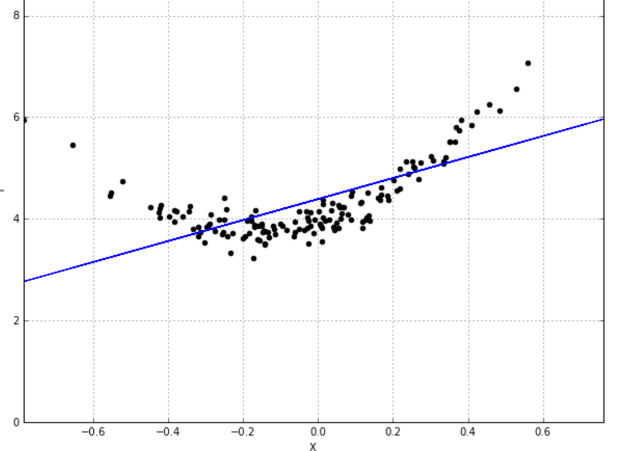
\includegraphics[scale=0.5]{problem} \pause

\begin{columns}
\begin{column}{7cm}

 $ y= \beta_0 + \beta_1 \cdot x + \beta_2 \cdot x^2 + \varepsilon$
\end{column}


\end{columns}


\end{frame}
%%%%%%%%%%%%%%%%%%%%%%%%%%%%%%%%%%%%
\begin{frame}

\frametitle{Problem linearne regresije}
\begin{columns}
\begin{column}{12cm}

\alert{Kaj če ne želim (ne znam) v naprej določiti števila parametrov?}
\begin{itemize}
\item Želimo upoštevati vse možne funkcije, ki se ujemajo z našimi podatki, ne glede na to, koliko parametrov vsebujejo.
\item Neparametrično = neskončno mnogo parametrov
\end{itemize}

\end{column}
\end{columns}
\end{frame}


%%%%%%%%%%%%%%%

\begin{frame}

\frametitle{Omejitev funkcij, ki jih želimo}
\begin{columns}
\begin{column}{12cm}

\begin{itemize}
\item Zaloga vrednosti
\item \alert{Gladkost}
\item Povprečna vrednost
\end{itemize}
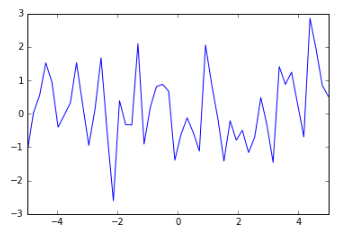
\includegraphics[scale=0.5]{vjuga}
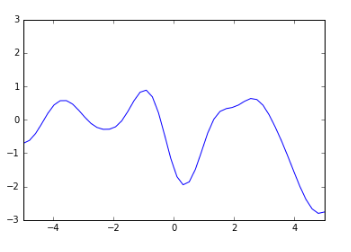
\includegraphics[scale=0.5]{gladka}
\end{column}


\end{columns}
\end{frame}

%%%%%%%%%
\begin{frame}

\frametitle{Gladkost}
\begin{columns}
\begin{column}{12cm}

\begin{itemize}
\item Podobne vrednosti vhodnih podatkov producirajo podobne vrednosti izhodnih
\item \alert{Kovariančna matrika} (kovariančna funkcija)

\end{itemize}

\end{column}


\end{columns}
\end{frame}
%%%%%%%%%
\begin{frame}

\frametitle{Prior in posterior}
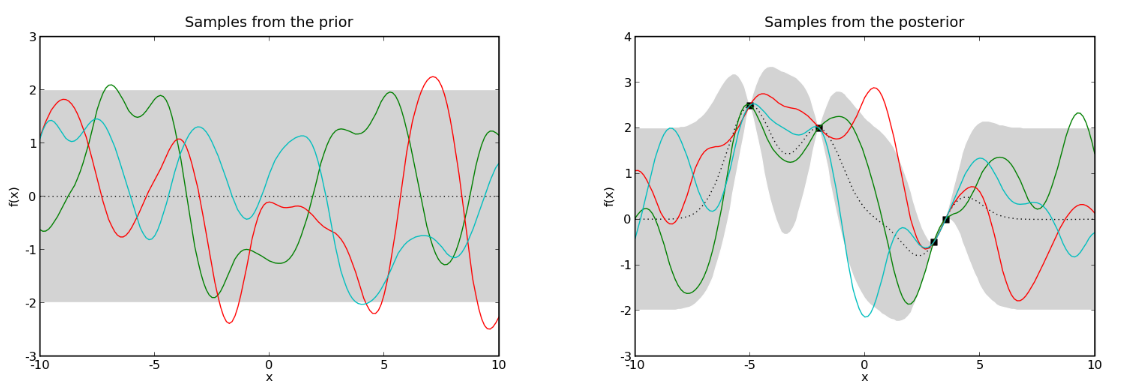
\includegraphics[scale=0.35]{pripost}

\end{frame}




%%%%%%%%%


\begin{frame}

\frametitle{Gaussov proces}

\begin{proposition} 
\alert{Slučajni proces} je zaporedje slučajnih spremenljivk $(X_t)_{t\ge0 } $.
\end{proposition}

\begin{proposition}
Slučajni proces $(X_t)_{t \in T } $ je \alert{Gaussov}, če je za katerokoli končno podmnožico $ F \subset T$, slučajni vektor $ X_F := (X_t)_{t \in F}$ (večrazsežno) normalno porazdeljen. 
\end{proposition}

Drugače: Slučajni proces je Gaussov, če je za vsak vektor neodvisnih spremenljivk $x$, vrednost funckije $f(x)$ porazdeljena po normalni (Gaussovi) porazdelitvi.
\end{frame}

%%%%%%%%%%%%%%%%%%
\begin{frame}

\frametitle{Gaussov proces}

Gaussov proces $f(x)$ je določen s funkcijo matematičnega upanja $m(x)$ in kovariančno funkcijo $k(x, x')$, kjer sta:
\begin{itemize}
\item $ m(x) = E[ f(x) ] $, 
\item $ k(x, x') = E[ (f(x) - m(x)) (f(x')-m(x')) ] $.
\end{itemize}

Pišemo: $ f(x) \sim \mathcal{GP}(m(x), k(x,x'))$.


\end{frame}

%%%%%%%%%%%%%%%%%%%%%%%%%%%
\begin{frame}

\frametitle{Kovariančna funkcija}

Vrednost kovariančne funkcije $k(x_i, x_j)$ izraža korelacijo med posameznima izhodoma $f(x_i)$ in $f(x_j)$ modela, obravnavana kot dve medsebojno povezani naključni spremenljivki. 
\begin{itemize}
\item $ k(x_i, x_j) = E[ (f(x_i) - m(x_i)) (f(x_j)-m(x_j)) ] $.
\end{itemize}




\end{frame}

%%%%%%%%%%%%%%%%

\begin{frame}

\frametitle{Primerjava različnih kovarianc}
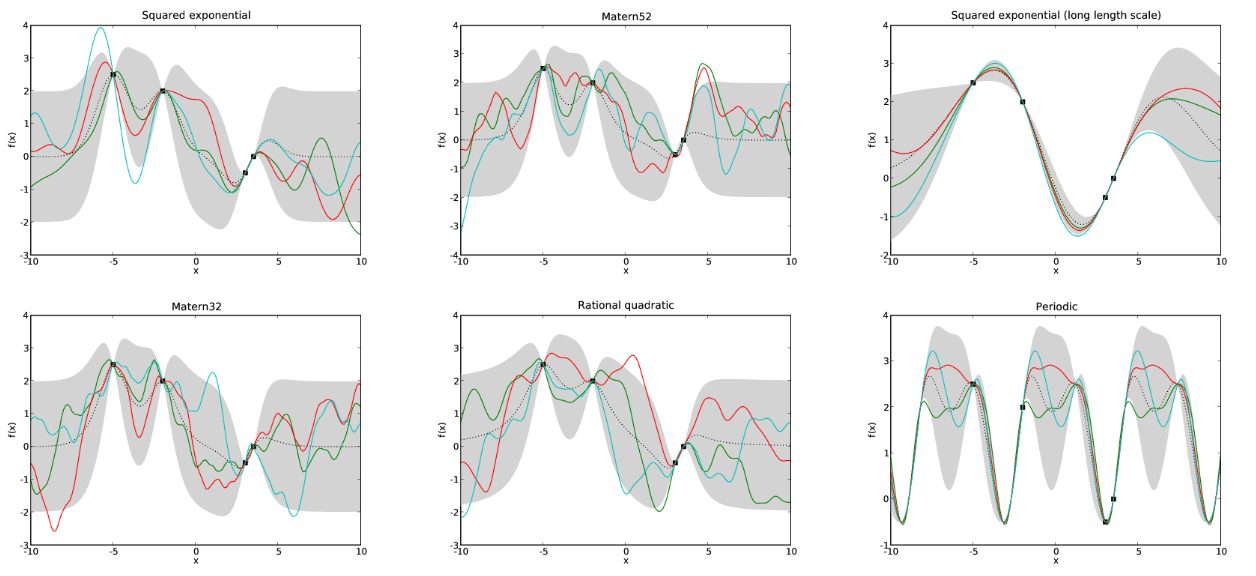
\includegraphics[scale=0.35]{kovariance}

\end{frame}
%%%%%%%%%%%%%%%%
\begin{frame}

\frametitle{GP model}

\begin{itemize}
\item \textbf{Predhodno znanje} (ang. \textit{prior}) odraža mnenje o preslikavi med vhodi in izhodi. Običajno predpostavlja gladkost.
\item \textbf{Posteriorno znanje} (ang. \textit{posterior}) dobimo, ko v model vključimo še končno število vhodno-izhodnih parov $(x_i, y_i)$.
Dobimo posteriorno porazdelitev za predikcijo modela. 
\item \textbf{Vhod} v GP model: posamezne vrednosti neodvisnih spremenljivk, zbrane v vhodnem vektorju x
\item \textbf{Izhod} iz GP modela: verjetnostna porazdelitev izhodne vrednosti $ f(x)$ pri danem vhodnem vektorju
\end{itemize}

\end{frame}

%%%%%%%%%%%%%%%%

\begin{frame}

\frametitle{Delo v nadaljevanju}
\begin{itemize}

\item Izbira kovariančne funkcije je ključnega pomena za delovanje GP modela.
\item Empirični del diplomske naloge

\end{itemize}


\end{frame}
%%%%%%%%%

\end{document}




